\documentclass[a4paper, 12pt]{article}
\usepackage[T2A]{fontenc}
\usepackage[utf8]{inputenc}
\usepackage[english, russian]{babel}
\usepackage{amssymb,amsmath,mathrsfs,amsthm}
\usepackage{graphicx}
%\usepackage[footnotesize]{caption2}
\usepackage{caption}

\usepackage{makecell}
\usepackage{array}
\usepackage{subfig}
\usepackage{indentfirst}
\usepackage[ruled, vlined, linesnumbered]{algorithm2e}
\usepackage{tikz}
\usetikzlibrary{shapes, arrows, calc}
\usepackage{float}

%\usepackage[document]{ragged2e}
%\usepackage[ruled,section]{algorithm}
%\usepackage[noend]{algorithmic}
%\usepackage[all]{xy}
% перевод algorithm2e
\SetKwInput{KwData}{Исходные параметры}
\SetKwInput{KwResult}{Результат}
\SetKwInput{KwIn}{Входные данные}
\SetKwInput{KwOut}{Выходные данные}
\SetKwIF{If}{ElseIf}{Else}{если}{тогда}{иначе если}{иначе}{конец условия}
\SetKwFor{While}{до тех пор, пока}{выполнять}{конец цикла}
\SetKw{KwTo}{от}
\SetKw{KwRet}{возвратить}
\SetKw{Return}{возвратить}
\SetKwBlock{Begin}{начало блока}{конец блока}
\SetKwSwitch{Switch}{Case}{Other}{Проверить значение}{и выполнить}{вариант}{в противном случае}{конец варианта}{конец проверки значений}
\SetKwFor{For}{для}{}{}
\SetKwFor{ForEach}{для каждого}{выполнять}{конец цикла}
\SetKwRepeat{Repeat}{повторять}{до тех пор, пока}
\SetAlgorithmName{Алгоритм}{алгоритм}{Список алгоритмов}
\SetArgSty{textnormal}
\SetCommentSty{textnormal}

\makeatletter
\newcommand{\nosemic}{\renewcommand{\@endalgocfline}{\relax}}% Drop semi-colon ;
\newcommand{\dosemic}{\renewcommand{\@endalgocfline}{\algocf@endline}}% Reinstate semi-colon ;
\newcommand{\pushline}{\Indp}% Indent
\newcommand{\popline}{\Indm\dosemic}%
\newcommand{\kNN}{\textrm{kNN}}
\newcommand{\argmax}{\textrm{argmax}}
\newcommand{\mean}{\textrm{mean}}

\addto\captionsenglish{\renewcommand{\figurename}{Рис.}}
\righthyphenmin=3
\emergencystretch=5pt
% \sloppy
% !TeX spellcheck = ru

\begin{document}

\begin{titlepage}
\begin{center}

    \bigskip
    \includegraphics[width=80mm]{msu.eps}

    Московский государственный университет имени М. В. Ломоносова
    Факультет Вычислительной Математики и Кибернетики \\
    Кафедра Математических Методов Прогнозирования \\

	\vspace{25mm}	

	{\large
    Коробов Павел Андреевич  \\[5mm]
    {\bfseries Обучение с подкреплением в задаче рекомендаций} \\[5mm]
    {\bfseries Reinforcement learning for recommender systems } \\[5mm]
         КУРСОВАЯ РАБОТА \\[10mm]
	}
		
	\vspace{25mm}	
	
    \begin{flushright}
            {\bfseries Научный руководитель:} \\
            н. с. Д. А. Кропотов
    \end{flushright}

    \vspace{\fill}
    Москва, 2020
\end{center}
\end{titlepage}

\newpage
\renewcommand{\contentsname}{Содержание}
\tableofcontents

%\newpage
%\begin{abstract}
%	В данной работе рассматривается применение алгоритмов обучения с подкреплением к задаче рекомендаций.  Классические методы построения рекомендаций, как правило, не учитывают своё влияние на дальнейшее поведение пользователей в отличие от алгоритмов обучения с подкреплением. Отсюда могут возникать негативные эффекты, такие как, например, пузырь фильтров.
%При этом методы обучения с подкреплением, основанные на явной максимизации Q-функции, такие как DQN, могут требовать слишком большой вычислительной сложности в том случае, если среда обладает большим пространством действий. Рекомендательная система должна быть способна справиться с такой задачей, ведь количество объектов для рекомендаций может достигать миллионов. Кроме того, DQN требует обучения на каждом действии пространства. Было бы хорошо иметь алгоритм способный близко оценивать похожие действия даже в том случае, когда он встречал только часть из них. В данной работе расматривается алгоритм Wolpertinger для работы с большими пространствами действий, изучаются условия его корректной работы и предлагается его модификация.
%\end{abstract}

\newpage
\section{Введение}

\subsection{Обучение с подкреплением}

Обучение с подкреплением -- это область машинного обучения,  в которой решается задача максимизации некоторой награды в ходе взаимодействий с окружающей средой. 

Окружающая среда в задаче обучения с подкреплением обычно задаётся марковским процессом принятия решений.
Это четвёрка $\left(\mathcal{S}, \mathcal{A}, \mathcal{P}, r\right)$, где:

\begin{itemize}
\item $\mathcal{S}$ -- пространство состояний
\item $\mathcal{A}$ -- пространство действий
\item $\mathcal{P}: \mathcal{S} \times \mathcal{R} \times \mathcal{S} \rightarrow \mathbb{R}^+$ -- функция переходных вероятностей $p\left(s^{\prime} | s, a\right)$
\item $r: \mathcal{ S } \times \mathcal { A } \rightarrow \mathbb{R}$ -- функция награды
\end{itemize} 
Система, отвечающая за выбор действий при взаимодействии со средой, называется агентом.  На рисунке \ref{fig:MDPscheme}  схематично изображена схема взаимодействия агента со средой. 

Сумма $R_{t}=\sum_{i=t}^{T} \gamma^{i-t} r\left(S_{i}, A_{i}\right)$ называется кумулятивной наградой.
Цель агента -- найти стратегию $\pi: \mathcal{S} \rightarrow \mathcal{A}$, максимизирующую ожидаемую кумулятивную награду $\mathbb{E}\left[R_1\right]$. Агенту неизвестны переходные вероятности и функция награды, он должен найти оптимальную стратегию методом проб и ошибок. 

\tikzstyle{block} = [draw, fill=blue!20, rectangle, 
    minimum height=3em, minimum width=6em]
\tikzstyle{sum} = [draw, fill=blue!20, circle, node distance=1cm]
\tikzstyle{input} = [coordinate]
\tikzstyle{output} = [coordinate]
\tikzstyle{pinstyle} = [pin edge={to-,thin,black}]
%

\tikzstyle{block} = [draw, fill=blue!20, rectangle, 
    minimum height=3em, minimum width=6em]
\tikzstyle{sum} = [draw, fill=blue!20, circle, node distance=1cm]
\tikzstyle{input} = [coordinate]
\tikzstyle{output} = [coordinate]
\tikzstyle{pinstyle} = [pin edge={to-,thin,black}]

\begin{figure}[h!]
	\centering

	\begin{tikzpicture}[auto, node distance=2cm,>=latex']

	    \node [block] (agent) {Агент};
    		\coordinate[right of=agent] (agent_right);
    		\coordinate[left of=agent] (agent_left);

  		\node [block, below of=agent] (env) {Среда};
    		\coordinate[right of=env] (env_right);
    		\coordinate[left of=env] (env_left);
    
    % Once the nodes are placed, connecting them is easy. 
    % right arrow
    		\draw[->](agent.east) -- (agent_right) -- node[above, sloped] {\tiny Действие $a_t$} (env_right) -- (env.east);
    % left external arrow
    		\draw[->]($(env.west) + (0.0, -0.2)$) -- ($(env_left) + (-1.0, -0.2)$) -- 
    				node[above, sloped] {\tiny Состояние $s_t$} ($(agent_left) + (-1.0, 0.2)$) -- ($(agent.west) + (0.0, 0.2)$);
	% left internal arrow
    		\draw[->]($(env.west) + (0.0, 0.2)$) -- node[above]{\tiny $r_{t+1}$} ($(env.west) + (-0.7, 0.2)$);
    		\draw[->]($(env.west) + (0.0, -0.2)$) -- node[below]{\tiny $s_{t+1}$}  ($(env.west) + (-0.7, -0.2)$);

    		\draw[->]($(env.west) + (0.0, 0.2)$) -- ($(env_left) + (-0.5, 0.2)$) -- 
    				node[above, sloped]{\tiny Награда $r_t$} ($(agent_left) + (-0.5, -0.2)$) -- ($(agent.west) + (0.0, -0.2)$);
    		\draw[densely dotted]($(env.west) + (-0.7, -0.6)$) -- ($(env.west) + (-0.7, 0.6)$);
	
	\end{tikzpicture}
	\caption{Схема марковского процесса принятия решений}
	\label{fig:MDPscheme}
\end{figure}

Q-функция состояний-действий $Q^{\pi}(s, a)=\mathbb{E}\left[R_{1}|S_{1}=s, A_{1}=a, \pi \right]$ оп\-ределяется как ожидаемая кумулятивная награда при условии начального состояния $s$, выбора действия $a$ и следования политике $\pi$.

% Для Q-функции верно следуещее равенство, называемое уравнением Беллмана:

%$$Q^{\pi}(s, a)=r(s, a)+\gamma \mathbb{E}_{s^{\prime} \sim p(s^{\prime} | s, a)} Q^{\pi} \left(s^{\prime}, \pi(s^{\prime})\right)$$



\subsection{Задача рекомендаций}

Пусть $M$ и $N$ -- числа пользователей и объектов соответственно.
Матрица $Y \in \mathbb{R}^{M \times N}$ хранит в себе оценки, выставленные объектам пользователями.  Компонента $y_{ij}$ соответствует оценке $i$-м пользователем $j$-го объекта. Наша цель -- предсказать для пользователей рейтинги непросмотренных ими объектов, то есть пропущенные значения в данной матрице, и рекомендовать пользователям объекты с наибольшим предсказанным рейтингом.

Как правило, эта задача формулируется как задача обучения с учителем, и её решение никак не учитывает влияние рекомендаций на поведение пользователей в долговременной перспективе. 

Существует известный эффект, присущий персонализированным сервисам, заключающийся в изоляции пользователей от разнообразия точек зрения.
Этот эффект называется пузырём фильтров, и рекомендательные сервисы потенциально подвержены этому эффекту. В \cite{filter_bubble} авторы показали, что разнообразие рекомендаций для пользователей сервиса рекомендаций фильмов MovieLens стало статистически значимо меньше в конце истории использования сервиса пользователем, чем оно было в начале.


Независимо от того, вызывается этот эффект естественно (например, тем, что хороших фильмов в целом не так много, и с большей персонализацией рекомендаций это множество только сужается) или недостатками алгоритма рекомендаций, обучение с подкреплением кажется более подходящей парадигмой для задачи рекомендаций, чем обучение с учителем.

Задача рекомендаций хорошо вписывается в концепцию обучения с подкреплением: оно явным образом учитывает поведение пользователей (реакцию среды) и максимизирует долгосрочную награду. Более того, в случае, если пользователь начнёт получать однообразные рекомендации, и его пользовательский опыт от этого начнет ухудшаться, мы можем надеяться, что агент, заметив ухудшение оценок пользователя, сможет найти более удачную стратегию, чем слишком подстраиваться под интересы пользователя, и в дальнейшем использовать этот опыт.

Кроме того, есть основания полагать, что с помощью алгоритмов обучения с подкреплением получится явно поддерживать разнообразие рекомендаций с помощью методов исследования среды. Например, этого можно достичь с помощью Maximum Entropy RL алгоритмов \cite{softq, sac}. 

\section{Постановка задачи}

Для оценки алгоритма обучения с подкреплением нужна среда или некоторый симулятор среды, на котором можно было бы убедиться в успешной работе алгоритма.
Мы будем использовать такой же симулятор среды для рекомендаций, как в оригинальной статье, представившей алгоритм Wolpertinger~\cite{wolpertinger}.

Предположим, что пользователи неразличимы и имеется некоторое множество объектов для рекомендаций, задающее пространство действий $\mathcal{A}$. Будем считать, что объекты из $\mathcal{A}$ некоторым образом пронумерованы. Пусть также задана матрица $W$, компоненты $w_{ij}$ которой задают вероятность принятия рекомендации $j$-го объекта при условии, что пользователь просматривает $i$-ый объект. 
За состояния принимаются объекты, просматриваемые пользователем в данный момент.
Таким образом,  $\mathcal{S}=\mathcal{A}$. 

Пользователь заканчивает эпизод с вероятностью $0.1$, если рекомендация была принята, и с вероятностью $0.2$ в противном случае. 
Если эпизод продолжается, в случае принятия рекомендации пользователь начинает просматривать рекомендованный объект, иначе равновероятно начинает просмотр любого из $\mathcal{A}$.

Несложно увидеть, что оптимальная политика является детерминированной и будет иметь вид $$\pi(s)=\argmax_j \{ w_{ij}~|~\text{$i$ --  номер текущего состояния $s$} \}.$$

По сути задача сводится к нахождению максимальных значений в строках матрицы $W$.
К сожалению, авторы~\cite{wolpertinger} не описали ни способа построения $W$ в своем эксперименте, ни способа построения эмбеддингов для объектов.

За основу эксперимента в данной работе были взяты данные конкурса The Netflix Prize.
В этом наборе данных содержится $24~053~764$ рейтингов на $17~770$ фильмов от $470~758$ пользователей.
Было решено строить матрицу $W$ и эмбеддинги для элементов $\mathcal{A}$ по этим данным.


Опишем, как задаётся матрица $W$.  Пусть $P_{ij}$ -- число положительных рейтингов фильма $j$, выставленных в течение $l$ дат позднее просмотра фильма $i$,  а $C_{ij}$ -- число всех рейтингов фильма $j$, выставленных в течение $l$ дат позднее просмотра фильма $i$.

 Для подсчета этих величин матрицы $P$ и $C$ инициализируются нулевыми матрицами, далее внутри истории каждого пользователя рейтинги разбиваются на даты. 
 
 Мы перебираем всех пользователей, и для текущего пользователя в цикле перебираем пары фильмов $(i, j)$ из его истории, где $i$ соответствует фильму, просмотренному в некоторую обрабатываемую в данный момент дату, а $j$ -- фильму, просмотренному в одну из следующих $l$ дат. При каждом нахождении такой пары $(i, j)$ среди историй всех пользователей мы увеличиваем счетчики $C_{ij} := C_{ij} + 1$, $P_{ij} := P_{ij} + b(r_{ij})$, где
 
$$
b(x)=
	\begin{cases}
		1 & \text{если } x > 3\\
		\frac12 & \text{если } x = 3\\
		0 & \text{иначе} 
	\end{cases}.
$$

Пусть также $p = \sum_r b(r)$, $c = \sum_r 1$ -- суммы по всем рейтингам $r$ в данных.

Наконец, будем определять компоненты $w_{ij} = \frac{P_{ij} + p}{C_{ij} + c}$.
То есть это доли положительных рейтингов, поставленных пользователями фильму $j$ в течение $l$ дат в их истории после просмотра фильма $i$. Такое определение вполне соответствует определению матрицы $W$ в эксперименте из \cite{wolpertinger}, где смысл величины $w_{ij}$ -- вероятность принятия рекомендации объекта $j$ при рассмотрении объекта $i$.
В качестве априорных вероятностей берётся доля положительных рейтингов среди всех рейтингов $\frac{p}{c}$.

Эмбеддинги расчитывались с помощью алгоритма Skip-gram \cite{skip_gram}, реализованного классом Word2Vec  библиотеки gensim. Для применения алгоритма к рекомендуемым объектам история пользователей трактуется как предложения, а объекты -- как слова. 


% Использовадись следующие гиперпараметры: размерность эмбеддингов $d$ была взята равной 20; размер окна, из которого сэмплируется контекст, равен 20; число негативных <<слов>> равно 5; 

% Важно, чтобы представления объектов в $\mathbb{R^d}$ 

\section{Методы}

\subsection{Алгоритм Wolpertinger}

Применение алгоритмов, основанных на явной максимизации Q-функ\-ции, таких как DQN \cite{dqn}, может быть затруднительно при решении задачи рекомендаций. 
Перебор всех возможных действий во время поиска максимума Q-функции может быть слишком вычислительно затратен, так как нередко от рекомендательных систем требуется способность делать выбор среди миллионов объектов.
К тому же, в случае DQN, нужно оценить Q-функцию на каждом действии из $\mathcal{A}$.  То есть только для оценки $Q(s, \cdot)$ при одном фиксированном $s$ алгоритму требуется как минимум $|\mathcal{A}|$ шагов. Хотелось бы, чтобы алгоритм имел чуть лучшие обобщающие свойства: если мы умеем оценивать Q-функцию для какого-то одного действия, то было бы хорошо иметь близкие её значения для похожих действий. 

Таким свойством обладают алгоритмы типа Actor-Critic для непрерывного контроля благодаря непрерывности критика.
Кроме того, алгоритмы этого класса избегают явной максимизации Q-функции. 

Алгоритм Wolpertinger \cite{wolpertinger} переносит алгоритм DDPG \cite{ddpg} на дискретное пространство действий. Дискретные действия представляются эмбеддингами из $\mathbb{R}^d$.
Wolpertinger использует актёра DDPG, которого будем обозночать как $f_{\theta^\pi}(\cdot)$, для выбора так называемых протодействий $\hat{a} = f_{\theta^\pi}(s)$ из 
$\mathbb{R}^d$. При этом $\hat{a}$ может вовсе не соответствовать ни одному действию из $\mathcal{A}$ . Поэтому алгоритм ищет $k$ ближайших соседей $\hat{a}$ из $\mathcal{A}$ и выбирает среди них действие наиболее высоко оцениваемое критиком. Таким образом формируется полная политика $\pi(\cdot)$ агента Wolpertinger, показанная в алгоритме \ref{alg:policy}.

\

{	\small
\begin{algorithm}[H]
	\SetAlgoLined
	Пусть $s$ -- состояние полученное из среды \\
	$\hat{a} = f_{\theta^\pi}(s)$ \tcp{Выбрать протодействие}
	$\mathcal{A}_k = \kNN_{\mathcal{A}} (\hat{a})$ \tcp{Найти $k$ ближайших действий из $\mathcal{A}$ к $\hat{a}$ }
	$a = \argmax_{a_j \in \mathcal{A}_k} Q_{\theta^{Q^{\prime}}} (s, a_j)$ \tcp{Выбрать итоговое действие}
	Применить действие $a$ к среде; получить $r$ и $s \prime$
\caption{Политика Wolpertinger}
\label{alg:policy}
\end{algorithm}
}

Алгоритм \ref{alg:wolpertinger} полностью описывает устройство Wolpertinger.
Критик обучается исключительно на полной политике $\pi(\cdot)$, в то время как актёр для дифференцируемости оптимизируется по частичной политике $f(\cdot)$. 

% Wolpertinger по своему принципу работы напоминает двухступенчатую рекомендательную систему \cite{two_stage}. В \cite{two_stage} сначала выбираются некоторые кандидаты для рекомендаций, которые в дальнейшем ранжируются для формирования итоговых рекомендаций. 


\begin{figure}[H]
	\captionsetup{font=scriptsize}
	\centering
    		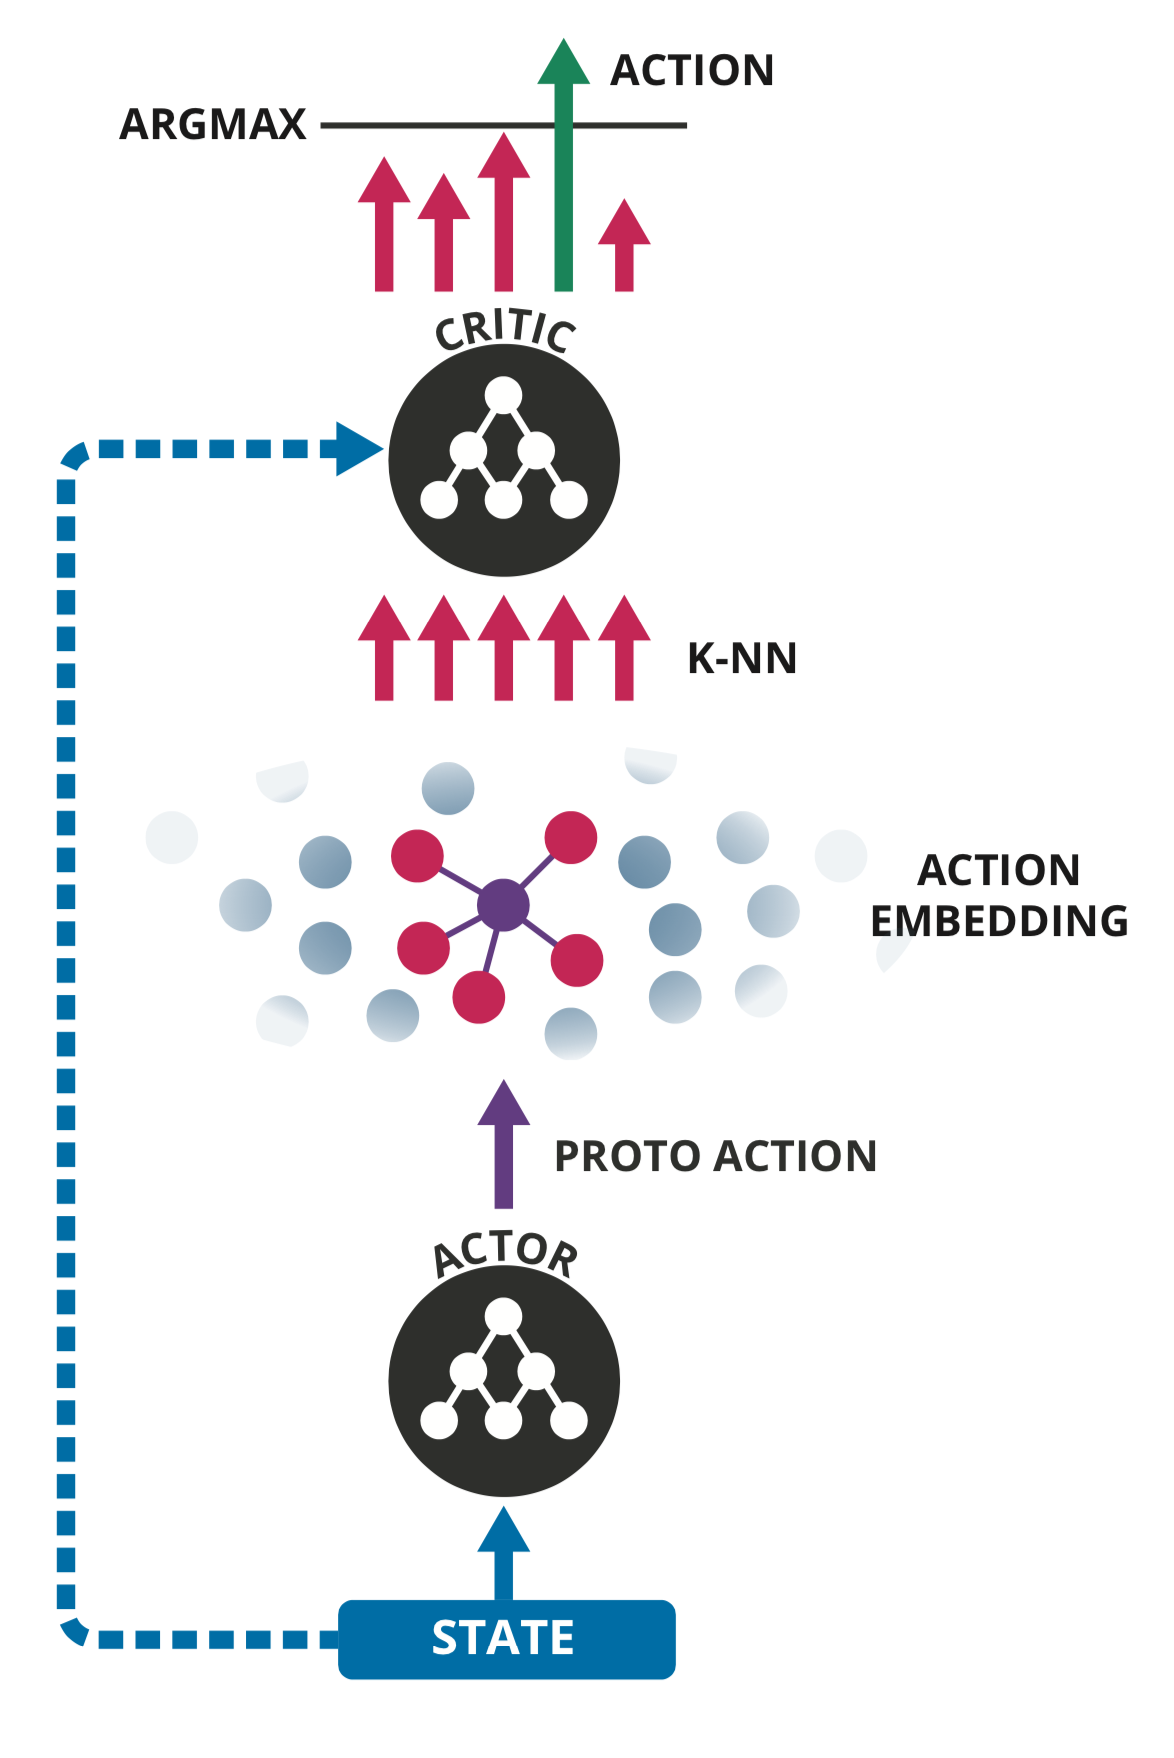
\includegraphics[width=.4\textwidth]{pics/wolpertinger}
   \captionsetup{justification=centering}
   \caption{Схема политики Wolpertinger}
\end{figure}

{	\small
\begin{algorithm}[H]
	\SetAlgoLined
	Инициализировать нейронные сети критика $Q_{\theta^Q}$ и актёра $f_{\theta^\pi}$ весами $\theta^Q$ и $\theta^\pi$ \\
	Инициализировать таргет-сети критика $Q_{\theta^{Q^\prime}}$ и актёра $f_{\theta^{\pi^\prime}}$ теми же весами 
	$\theta^{Q^\prime} \leftarrow \theta^Q$, 
	$\theta^{\pi^\prime} \leftarrow \theta^\pi$ \\
	Инициализировать буффер памяти $B$ \\
	\For{эпизода $e = 1, M$}{
		
		Получить начальное состояние $s_1$ \\
		\For{$t = 1, T$}{
			Выбрать действие $a_t = \pi_\theta(s_t)$ согласно текущей 
			политике и методу  исследования среды \\
			Отдать в среду $a_t$, пронаблюдать $r_t$ и  $s_{t+1}$ \\
			Сохранить кортеж $(s_t, a_t, r_t, s_{t+1})$ в буфер $B$ \\
			Семплировать из $B$ минибатч из $N$ кортежей $(s_i, a_i, r_i, s_{i+1})$ \\
			Присвоить 
			$y_{i}=r_{i}+\gamma \cdot Q_{\theta^{Q^{\prime}}}\left(s_{i+1}, \pi_{\theta^{\prime}}(s_{i+1})\right)$ \\
			Обновить веса критика, минимизируя невязку $L\left(\theta^{Q}\right)=\frac{1}{N} \sum_{i}\left[y_{i}-Q_{\theta^{Q}}\left(s_{i}, a_{i}\right)\right]^{2}$ \\
			Обновить веса актёра, сделав шаг по градиенту политики
			$g_{\pi} \approx \left.\left.\frac{1}{N} \sum_{i} \nabla_{a} Q_{\theta^{Q}}(s, a)\right|_{a=f_{\theta^{\pi}}\left(s_{i}\right)} \nabla_{\theta^{\pi}} f_{\theta^{\pi}}(s)\right|_{s=s_i}$ \\
			Обновить таргет-сети: \\
			~~$\theta^{Q^{\prime}} \leftarrow \tau \theta^{Q}+(1-\tau) \theta^{Q^{\prime}}$ \\
			~~$\theta^{\pi \prime} \leftarrow \tau \theta^{\pi}+(1-\tau) \theta^{\pi \prime}$
		}
	}
\caption{Wolpertinger}
\label{alg:wolpertinger}
\end{algorithm}
}

Авторы предлагают использовать приближенный поиск ближайших соседей, но чтобы убедиться в корректной работе алгоритма, мы будем искать соседей точно.

\subsection{Модификация Wolpertinger}

Непрерывность функции критика $Q_{\theta^Q}(s, \cdot)$ по действиям и её оценивание лишь в точках, заданных эмбеддингами действий из $\mathcal{A}$, может привести к тому, что протодействия, удаленные от множества $\mathcal{A}$ могут ошибочно максимизировать $Q_{\theta^Q}(s, \cdot)$. Это может спровоцировать нежелательное поведение актёра выбирать протодействия, находящиеся в областях, где критик элементарно не обучен ни на какие значения. Непрерывность критика может помочь близко оценивать похожие протодействия лишь в некоторых окрестностях точек $a \in \mathcal{A}$, чего может быть недостаточно в случае неплотного размещения эмбеддингов в $\mathbb{R}^d$.

Мы покажем, что $l_2$-регуляризация сетей вместе с использованием описанного в уравнении \ref{eq:neighbour_loss} добавочного слагаемого в функции потерь может существенно улучшить результаты работы алгоритма. 
Мы попробуем регуляризовать функцию потерь критика следующим образом:

\begin{equation}
\label{eq:neighbour_loss}
L\left(\theta^{Q}\right):=\frac{1}{N} \sum_{i}\left[y_{i}-Q_{\theta^{Q}}\left(s_{i}, a_{i}\right)\right]^{2} + 
\frac{1}{N} \sum_{i}\left[Q_{\theta^{Q}}\left(s_{i}, \hat{a}_{i}\right) - Q_{\theta^{Q}}\left(s_{i}, \textrm{1NN} \left(\hat{a}_{i} \right)\right)]^{2} \right.
\end{equation}

Второе слагаемое несёт следующий смысл: даже если рассматриваемая точка $\hat{a}$ находится далеко от множества $\mathcal{A}$, мы хотим, чтобы значение в этой точке не превышало значения на ближайшей точке из этого множества. Таким образом, при оптимизации функции потерь актёра $J(\theta^\pi) = Q(s, \pi_{\theta^\pi}(s))$, должна снизиться вероятность того, что актёр обучится выбирать слишком далёкие точки в качестве протодействий. 

\section{Эксперименты}

Взглянем на средние значения кумулятивных наград. Будем проводить эксперимент в течение 500 000 шагов взаимодействия со средой. На графиках будем изображать среднюю награду за каждые 500 шагов. Для каждого агента будем проводить по три запуска эксперимента и усреднять получаемые графики, отображая средние по запускам значения и коридор стандартного отклонения.

Первые 50000 шагов алгоритм накапливает опыт, выбирая случайные действия, далее исследование среды проводится $\varepsilon$-жадно с $\varepsilon=0.05$, $\gamma = 0.99$, $\tau=0.001$, размер буффера памяти равен 500000, так что он хранит весь опыт в течение эксперимента.

Везде используются полносвязные нейронные сети с тремя скрытыми слоями и 256 скрытыми нейронами. На выходах критика и актёра находятся линейная активация и гиперболический тангенс соответственно. После каждого внутреннего слоя используется ReLU-активация. Размерность эмбеддингов действий равна 20,
$\text{learning\_rate}=0.0003$ для обеих сетей, $\text{batch\_size}=128$.

Мы возьмём небольшое пространство действий: $|\mathcal{A}| = 100$, чтобы можно было легче оценивать работу алгоритма. Будем рассматривать алгоритм Wolpertinger, использующий в политике 10 ближайших действий (10NN Wolpertinger), так как согласно результатам \cite{wolpertinger} алгоритм, использующий $10\%$ ближайших действий, наиболее сопоставим с использованием $100\%$.

В первую очередь, хочется отметить, что регуляризация положительно влияет на обучение, даже если актёр не влияет на работу алгоритма: это полезно для критика. Если мы будем рассматривать Wolpertinger, использующий все $|\mathcal{A}|=100$ ближайших действий, мы по сути перейдем к варианту Q-learning, так как выбор протодействий актёром не будет влиять на конечный выбор действия.
Стоит отметить, что даже в таком случае у Wolpertinger может остаться преимущество обобщения значений критика на похожих действиях. Однако, это может и наоборот мешать корректно оценивать Q-функцию, если действия приводящие к совершенно разной награде, имеют близкие эмбеддинги. Поэтому выбор эмбеддингов действий важен.
И для критика, и для актёра будем использовать коэффициент регуляризации, равный $0.001$.

Как видим на рисунке \ref{fig:100NN}, алгоритм не смог найти оптимальную политику, хотя и способен получать награду существенно более высокую, чем случайный алгоритм. Регуляризация помогает раньше получить более высокую награду, но со временем получаемые награды стали примерно равны.

\begin{figure}[H]
	\captionsetup{font=scriptsize}
	\centering
    		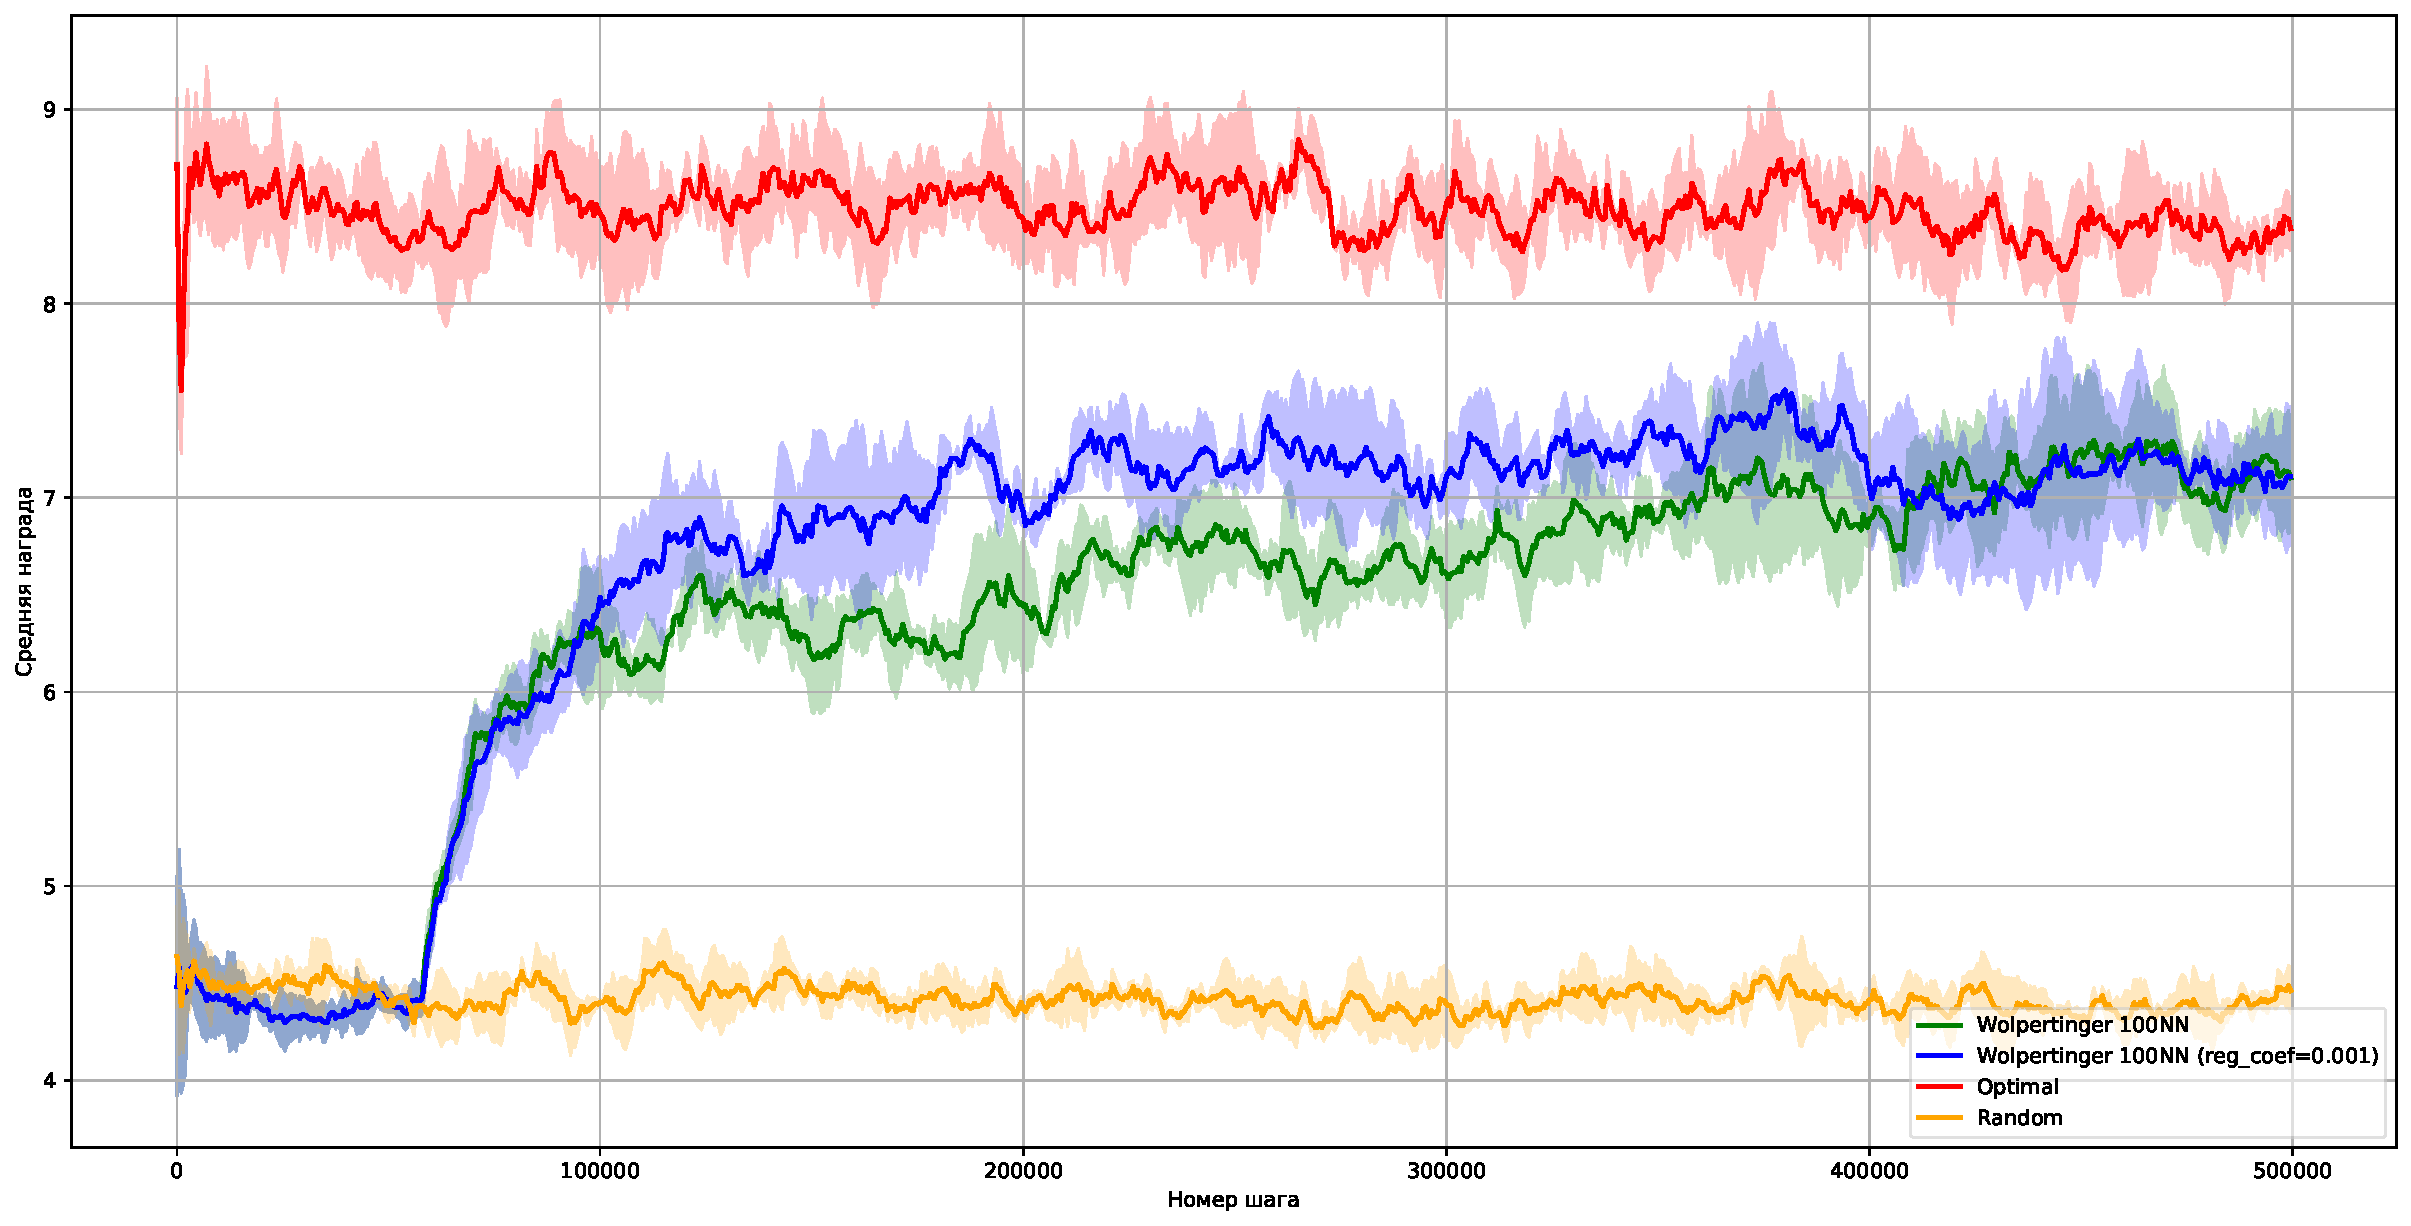
\includegraphics[width=1.0\textwidth]{pics/100NN.pdf}
   \captionsetup{justification=centering}
   \caption{Wolpertinger, использующий в политике $|\mathcal{A}|=100$ ближайших действий}
   \label{fig:100NN}
\end{figure}

Гланый интерес представляет случай, когда актёр включается в работу алгоритма. Мы видим на рисунке \ref{fig:10NN}, что алгоритм, не использующий $l_2$-регуляри\-зацию или регуляризацию с помощью ближайшего соседа даёт результаты сильно хуже, чем 100NN Wolpertinger. Но в случае, если мы добавим $l_2$-регуляризацию, мы получим очень близкие графики. Если дополнительно добавить к функции потерь критика слагаемое из уравенения \ref{eq:neighbour_loss}, мы получим синюю кривую, лежащую на графике выше всех остальных. Таким образом, получен алгоритм с достигающий награды даже большей, чем 100NN Wolpertinger.

Поясним, почему 10NN Wolpertinger с NN-регуляризацией может иметь наилучшие результаты.
Если взглянуть на значения растояний от протодействий до оптимальных действий $$\delta_s =  \|f_{\theta^\pi}(s) - a_{optimal} (s) \|_2,$$ 
получим следующие статистики:

\begin{center}
\setcellgapes{5pt}
\makegapedcells
\begin{tabular}{|c | c | c | c|} 
 \hline
  & Без регуляризации & $l_2$ & $l_2$ + NN \\
 \hline
 $\frac{1}{\mathcal{S}} \sum_{s \in \mathcal{S}} \delta_s$ & 1.962 & 1.927 & 1.164 \\ 
 \hline
  $\min_{s \in \mathcal{S}} \delta_s$ & 1.598 & 1.675 & 0.484 \\
 \hline
  $\max_{s \in \mathcal{S}} \delta_s$ & 2.146 & 2.278 & 1.788 \\
 \hline
\end{tabular}
\end{center}

Судя по третьему столбцу таблицы, вариант одновременной $l_2$ и NN-регуляризации помогает актёру выбирать протодействия существенно более близкие к оптимальным действиям.  
Возможно, что адекватный выбор протодействий вместе с максимизацией по меньшему числу соседей в политике позволяет в меньшей мере следовать неверным оценкам критика, которые имели место в случае 100NN Wolpertinger.

Минимальное и максимальное расстояния между парами используемых ембеддингов составляют 1.658 и 0.213 соответственно, откуда можно заключить, что первые два алгоритма из таблицы выдают крайне далёкие от множества $\mathcal{A}$ протодействия.

\begin{figure}[H]
	\captionsetup{font=scriptsize}
	\centering
    		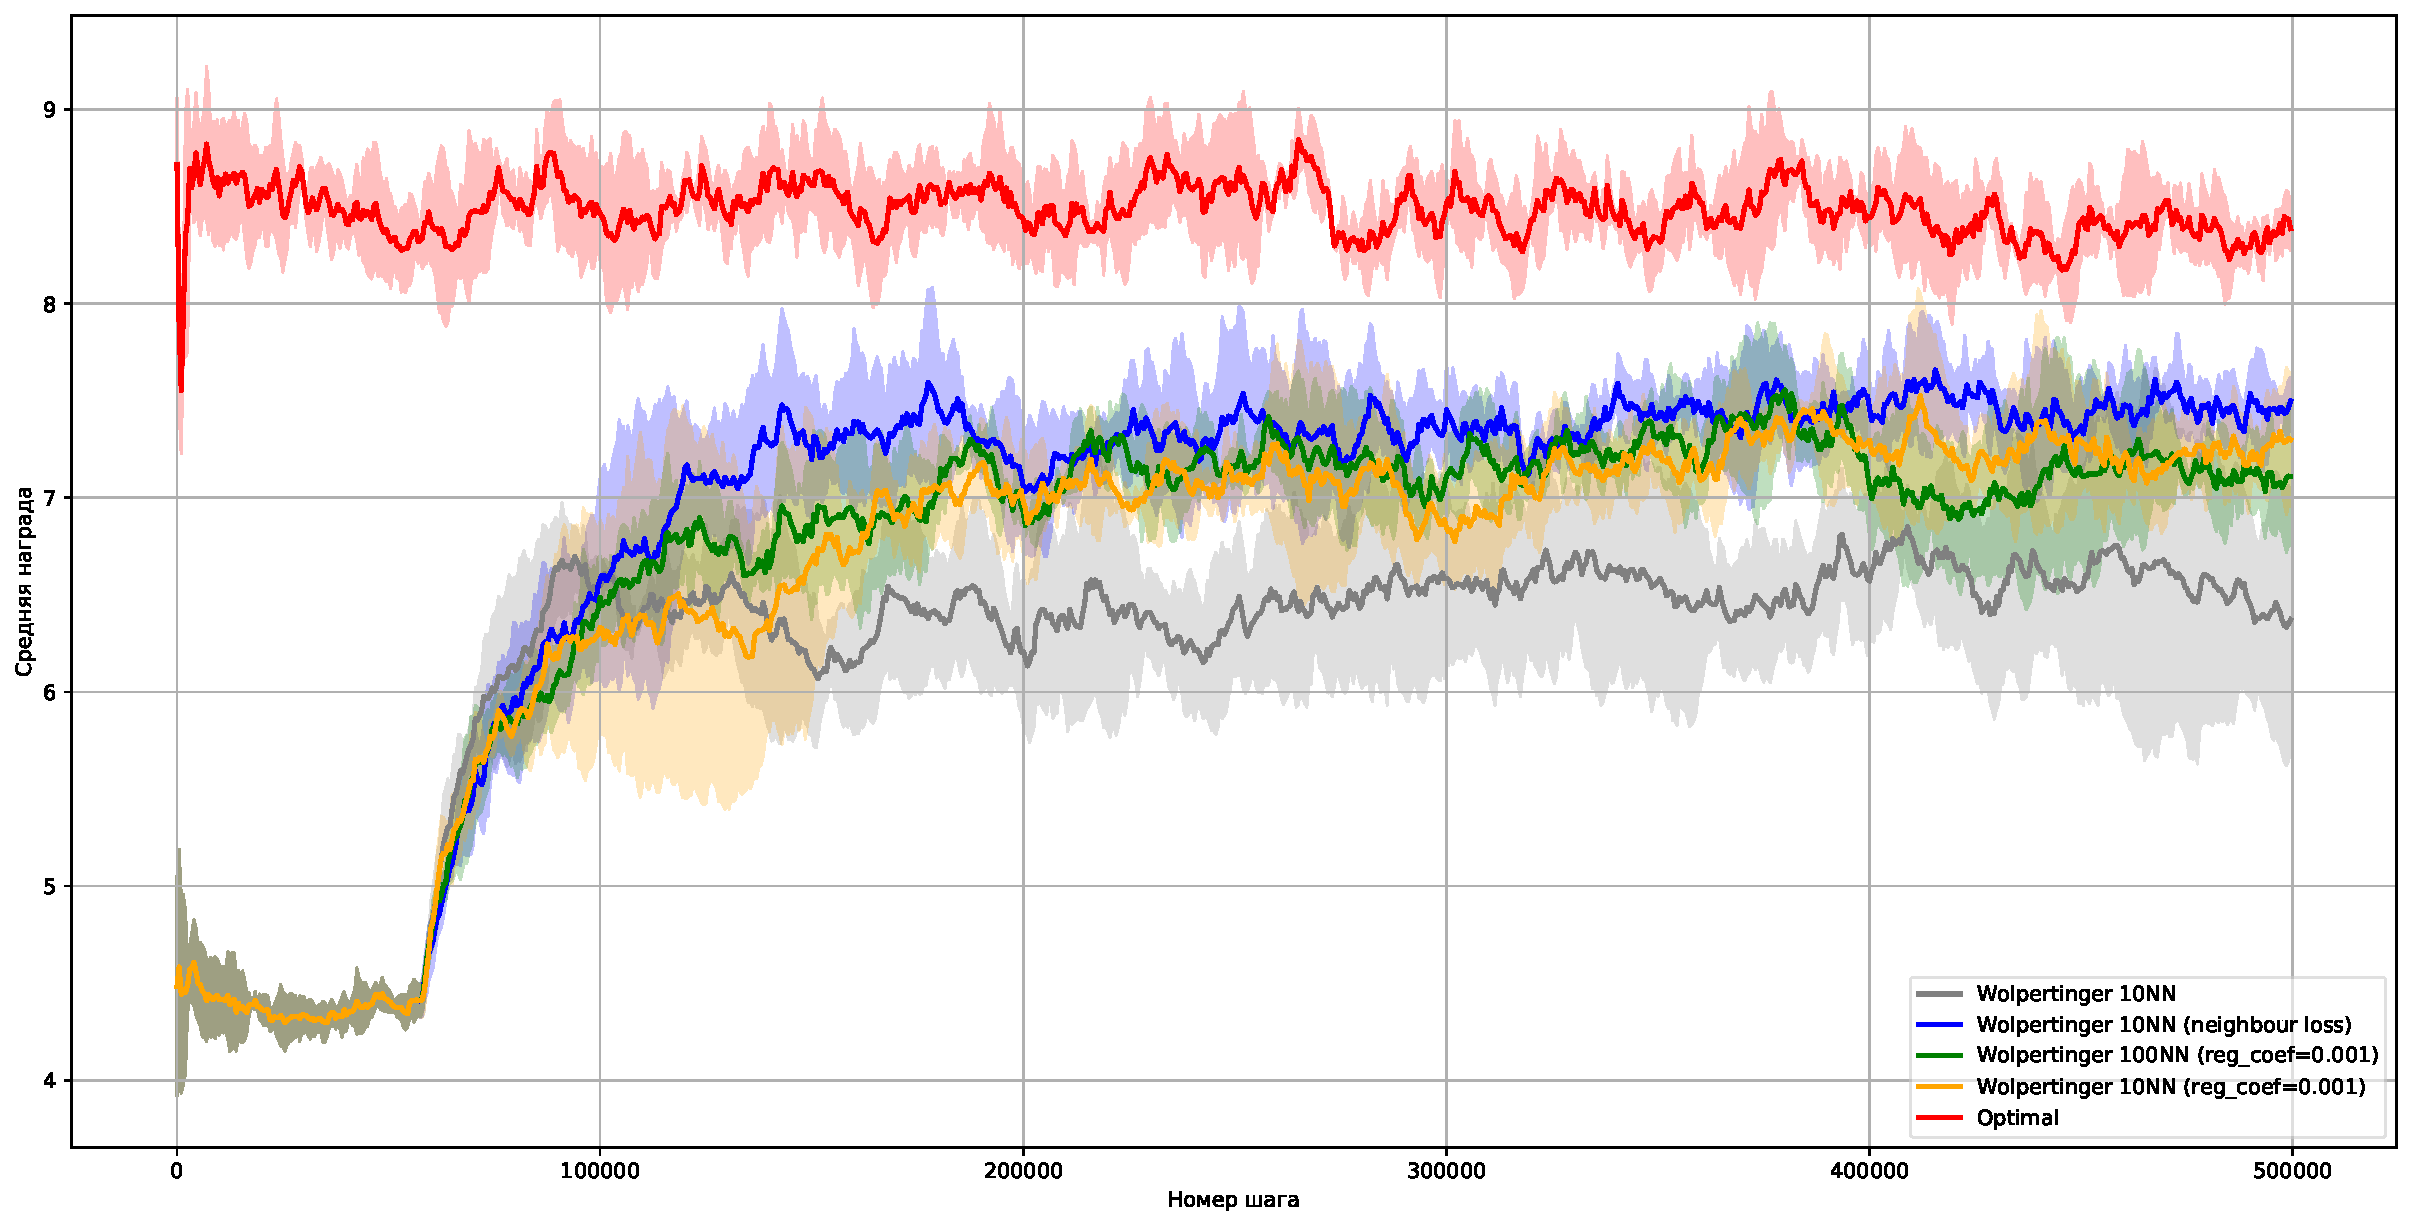
\includegraphics[width=1.0\textwidth]{pics/10NN.pdf}
   \captionsetup{justification=centering}
   \caption{Wolpertinger, использующий в политике $10$ ближайших действий}
   \label{fig:10NN}
\end{figure}

Взглянем, как расположены протодействия, выбранные для некоторых случайных состояний. Рассмотрим проекции действий и протодействий на первые пять осей.
Как видно по рисунку \ref{fig:projections}, версии алгоритма без NN-регуляризации склонны выбирать протодействия в сильно удаленных от $\mathcal{A}$ точках. Критик $Q_{\theta^Q}(s, \cdot)$ может иметь практически любые значения в точках, расположенных на большом расстоянии от $\mathcal{A}$, так как ни на что явно не обучается рядом с ними. Таким образом, актёр становится практически бесполезным и может в итоге просто всегда выбирать одну точку, далее выбор действия лишь как-то корректируется критиком, что не даёт выбирать совсем провальные действия.

В случае NN-регуляризации также видна тенденция к скучиванию точек и их удаленности, но в гораздо меньшей мере. Стоит при этом учитывать, что этот положительный эффект наблюдается по каждому измерению пространства эмбеддингов, из-за чего и сильно уменьшается среднее расстояние до оптимальных действий.

Не очень понятно, почему одна лишь $l_2$-регуляризация помогла, пусть и в меньшей степени, достичь большей награды. Как мы видим, на актёра это практически не подействовало. Видимо, это помогло лучшим образом обучить критика и выбирать лучшее из 10 ближайших действий.


\begin{figure}[H]
	\captionsetup{font=scriptsize}
	\centering
	\begin{tabular}[c]{cc}
		\subfloat{
    		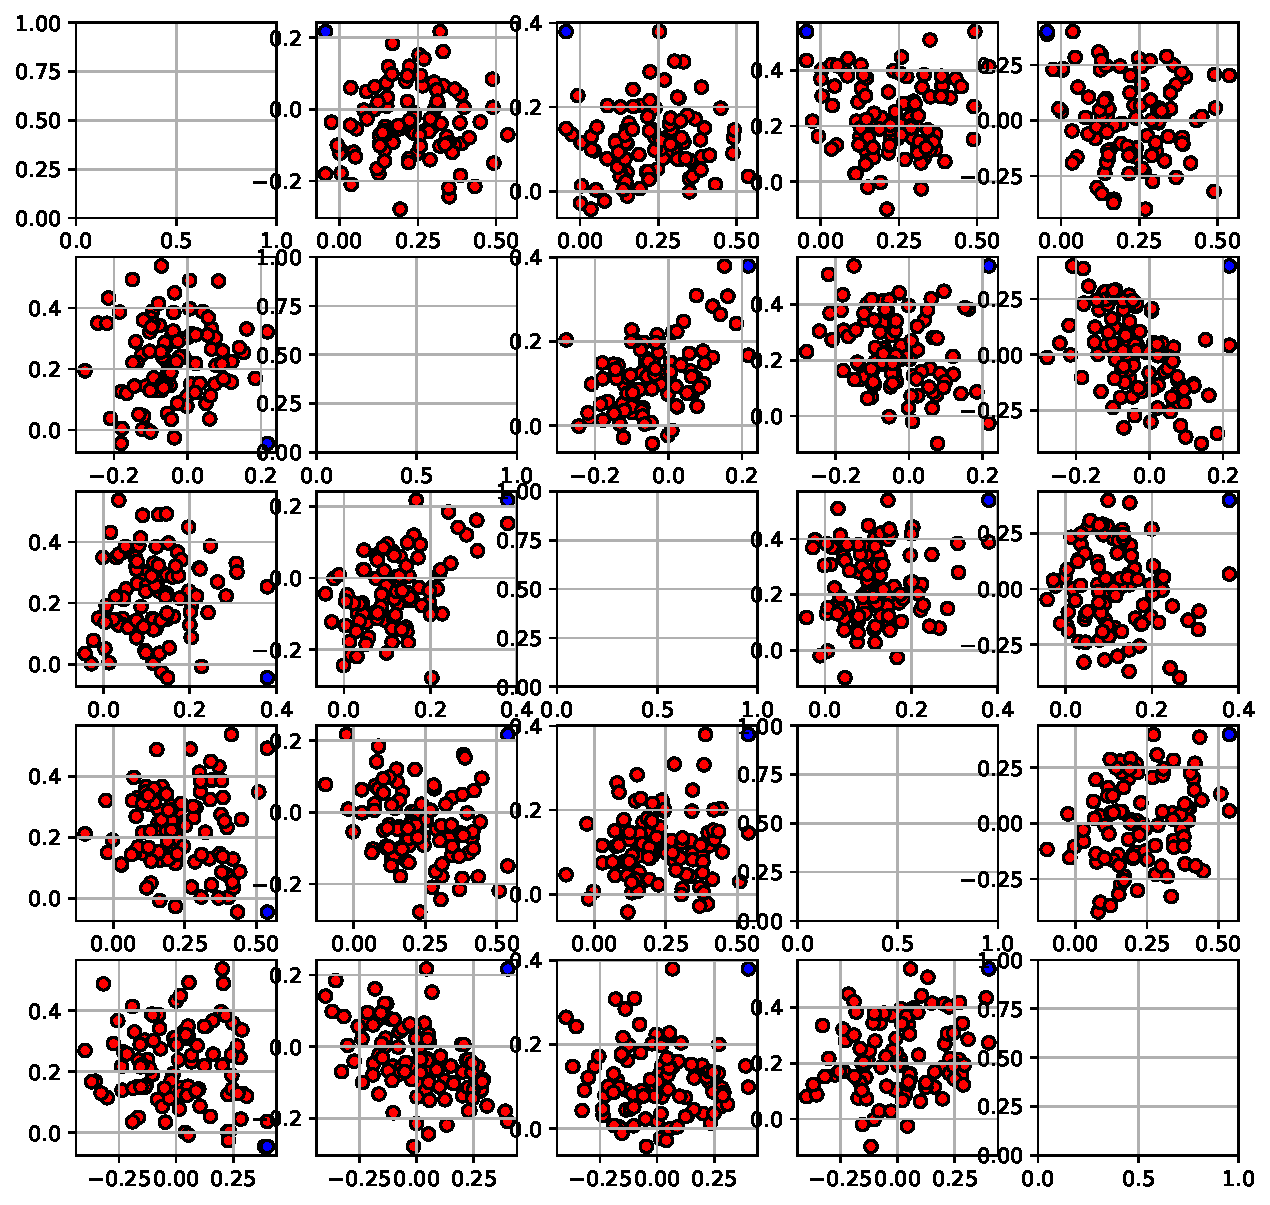
\includegraphics[width=.4\textwidth]{pics/proto_ordinary.pdf}
 		} &

		\subfloat{
    		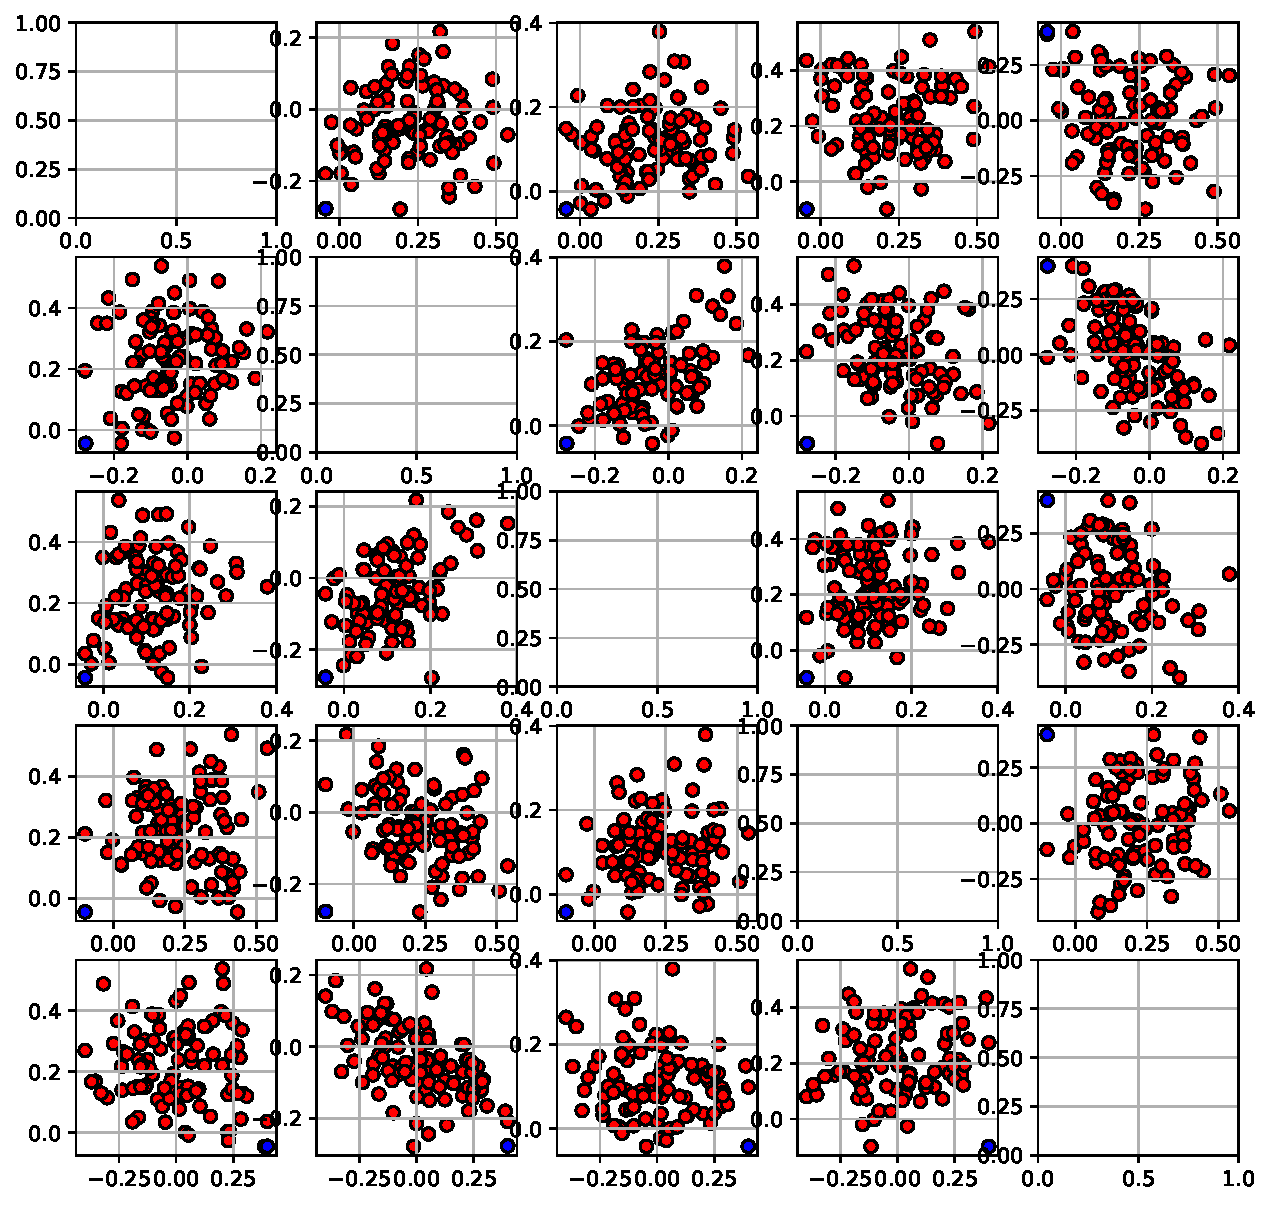
\includegraphics[width=.4\textwidth]{pics/proto_reg.pdf}
 		} 
    \end{tabular}
 	\subfloat{
    	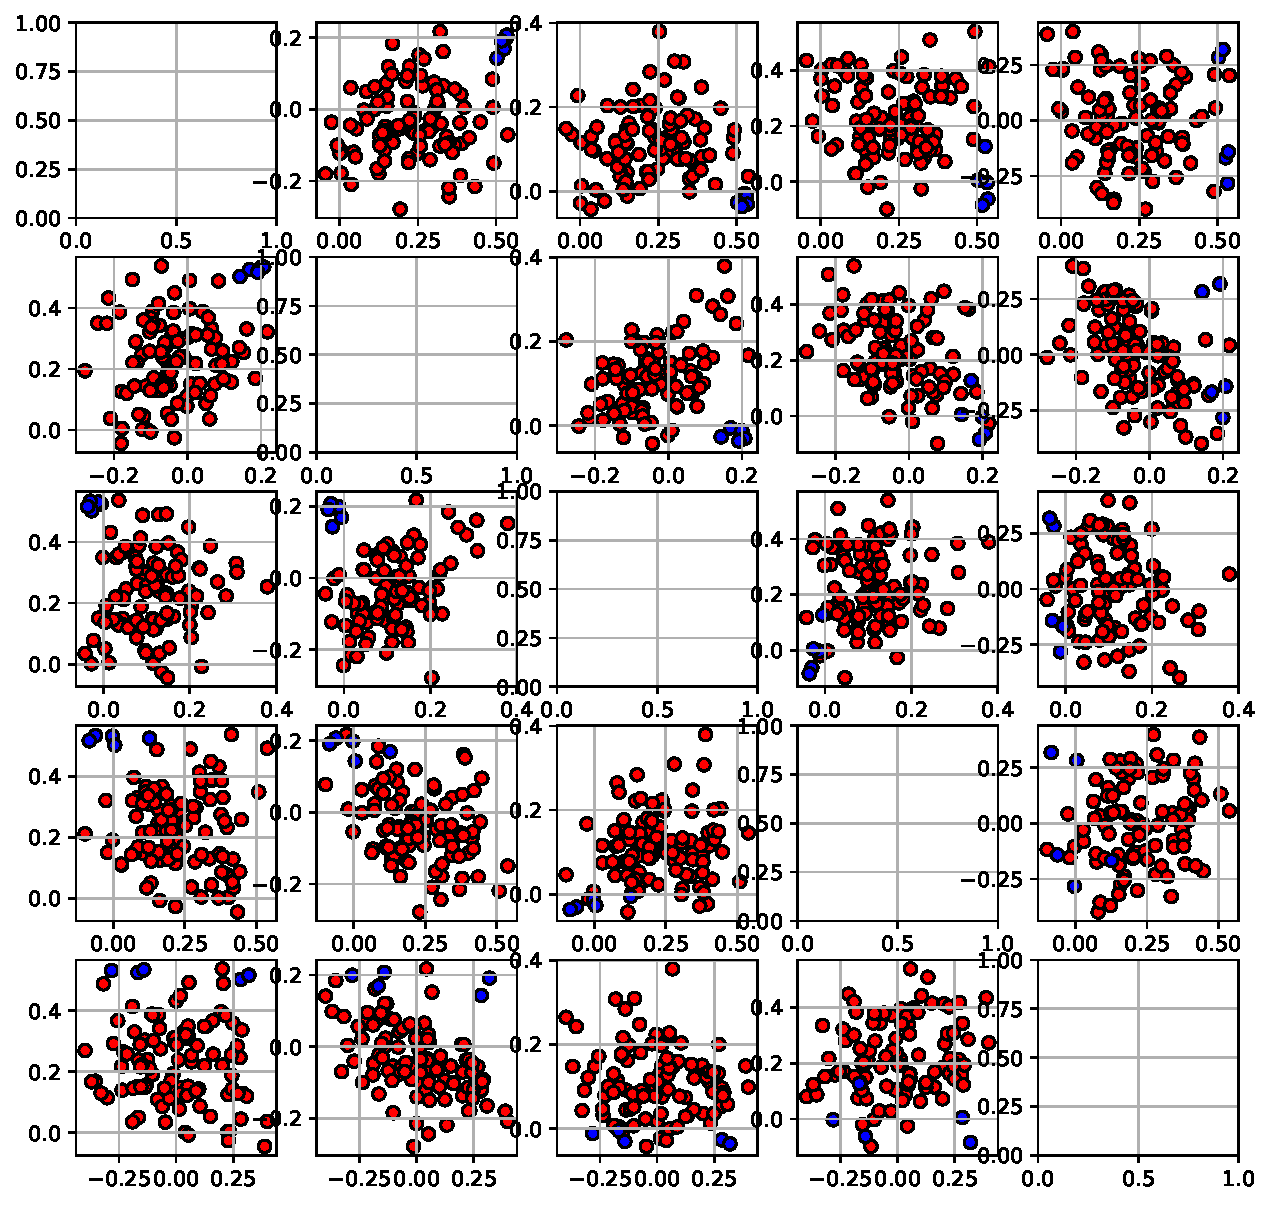
\includegraphics[width=.4\textwidth]{pics/proto_nn.pdf}
 }
   \captionsetup{justification=centering}
   \caption{Красным изображены проекции эмбеддингов на первые пять осей, синим -- протодействия в 5 одинаковых для каждого алгоритма случайных состояниях}
\label{fig:projections}
\end{figure}

\section{Заключение}

В данной работе был воспроизведён эксперимент из \cite{wolpertinger}. Была построена среда, подобная среде из оригинального эксперимента. Было показано, что во время обучения может возникнуть проблема зацикливания актёра на нерелевантных протодействиях из-за оптимизации критика только на пространстве действий. Была предложена модификация функции потерь критика, которая способна исправить эту проблему.

\newpage

% Возможно стоит добавить Sutton Barto, Top k off policy reinforce
% https://storage.googleapis.com/pub-tools-public-publication-data/pdf/45530.pdf
% http://wwwconference.org/proceedings/www2014/proceedings/p677.pdf/261960194_Exploring_the_filter_bubble_The_effect_of_using_recommender_systems_on_content_diversity

\renewcommand{\bibname}{Список литературы}
\addcontentsline{toc}{section}{\bibname}

\nocite{filter_bubble, barto_sutton,
			wolpertinger, 
			softq,
			sac}
%\def\BibUrl#1.{}\def\BibAnnote#1.{}
%\def\BibUrl#1{\\{\footnotesize\tt\def~{\char126} http://#1}}

% \bibliographystyle{unsrt}
\bibliographystyle{unsrt}
\bibliography{references}

% \cite{lamport94}

%\begin{thebibliography}{9} 
%\bibitem{lamport94} Leslie Lamport, \emph{\LaTeX: a document preparation system}. Addison Wesley, Massachusetts, 2nd edition, 1994. 
%
%\bibitem{filter_bubble} Tien T. Nguyen et al. Exploring the Filter Bubble: The Effect of Using Recommender Systems on Content Diversity // WWW 2014 Proceedings, pages 677–686, 2014. 
%
%\bibitem{softq} Tuomas Haarnoja, Haoran Tang, Pieter Abbeel, and Sergey Levine. Reinforcement Learning with Deep Energy-Based Policies. 

% arXiv e-prints, page arXiv:1702.08165, February 2017.

%\end{thebibliography} 

\end{document}
